\hypertarget{development-of-reactive-machine-models---initialisation}{%
\section{Development of Reactive Machine Models -
Initialisation}\label{development-of-reactive-machine-models---initialisation}}

\begin{itemize}
\tightlist
\item
  Every state-diagram must have exactly one initial state
\item
  But a technical process can be in any state, at the moment the
  embedded system is switched on
\item
  In order to have a correspondence between technical process state and
  embedded system state, they must be synchronised at start up. This can
  be done

  \begin{itemize}
  \tightlist
  \item
    By forcing the technical process to the assumed initial state at
    start up
  \item
    By introducing dedicated events to bring the embedded system into
    the state of the technical process
  \end{itemize}
\end{itemize}

\hypertarget{dedicated-init-state}{%
\subsection{Dedicated init state}\label{dedicated-init-state}}

\begin{itemize}
\tightlist
\item
  Introduction of a specific Init-States (ordinary state).
\item
  In the Init-State an init event-message is expected.
\item
  The transitions triggered by init messages lead to the correct state
  of the embedded system.
\end{itemize}

\textbf{The init-messages}

\begin{itemize}
\tightlist
\item
  Inform about the state of the technical process on start up
\item
  Are part of the virtual interaction.
\item
  Are generated by the embedded connection.
\item
  There are no corresponding events of the technical process.
\item
  Every reactive-object receives at most one init-message during its
  live time (live time ends when the system is turned off).
\end{itemize}

\begin{figure}[H]
\centering
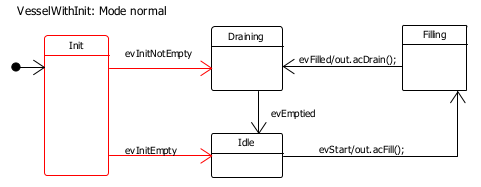
\includegraphics[width=0.8\textwidth]{figures/developmentReactiveMachineModelInit.png}
\caption{New init state}
\end{figure}

\hypertarget{complex-initialisation}{%
\subsection{Complex Initialisation}\label{complex-initialisation}}

\begin{itemize}
\tightlist
\item
  Initialisation of a system with more than one object.
\item
  A controller-object has to wait for other objects to be initialised.
\item
  The controller enters the state Run only if all other objects have
  finished initialisation.
\item
  Introduction of a gate isInitialized, which becomes true, if all other
  objects are initialised.
\end{itemize}

\begin{figure}[H]
\centering
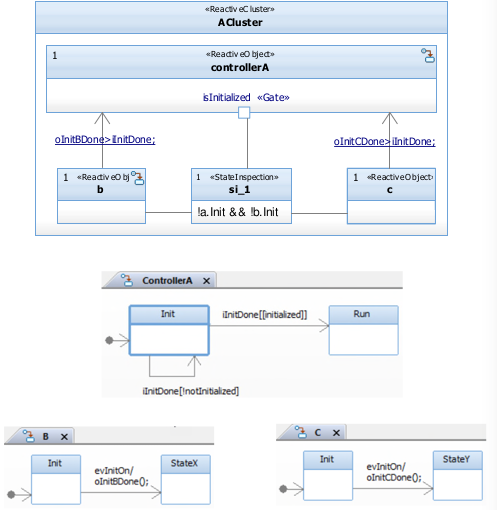
\includegraphics[width=1\textwidth]{figures/developmentReactiveMachineModelInit2.png}
\caption{Complex initialisation}
\end{figure}
